\documentclass[conference]{IEEEtran}
\IEEEoverridecommandlockouts
% The preceding line is only needed to identify funding in the first footnote. If that is unneeded, please comment it out.
\usepackage{cite}
\usepackage{amsmath,amssymb,amsfonts}
\usepackage{algorithmic}
\usepackage{graphicx}
\usepackage{textcomp}
\usepackage{xcolor}
\usepackage{svg}
\usepackage{multirow}
\usepackage{rotating}
\usepackage{mdframed}
\usepackage{hyperref}
\usepackage{tikz}
\usepackage{makecell}
\usepackage{tcolorbox}
\usepackage{amsthm}
%\usepackage[english]{babel}
\usepackage{pifont} % checkmarks
%\theoremstyle{definition}
%\newtheorem{definition}{Definition}[section]

\usepackage{listings}
\lstset
{ 
    basicstyle=\footnotesize,
    numbers=left,
    stepnumber=1,
    xleftmargin=5.0ex,
}


%SCJ
\usepackage{subcaption}
\usepackage{array, multirow}
\usepackage{enumitem}


\def\BibTeX{{\rm B\kern-.05em{\sc i\kern-.025em b}\kern-.08em
    T\kern-.1667em\lower.7ex\hbox{E}\kern-.125emX}}
\begin{document}
\pagestyle{plain} % Tilføjer page number på bottom of page
%\IEEEpubid{978-1-6654-8356-8/22/\$31.00 ©2022 IEEE}
% @Sune:
% Found this suggestion: https://site.ieee.org/compel2018/ieee-copyright-notice/
% I have added it - you can see if it fulfills the requirements

%\IEEEoverridecommandlockouts
%\IEEEpubid{\makebox[\columnwidth]{978-1-6654-8356-8/22/\$31.00 ©2022 IEEE %\hfill} \hspace{\columnsep}\makebox[\columnwidth]{ }}
                                 %978-1-6654-8356-8/22/$31.00 ©2022 IEEE
% copyright notice added:
%\makeatletter
%\setlength{\footskip}{20pt} 
%\def\ps@IEEEtitlepagestyle{%
%  \def\@oddfoot{\mycopyrightnotice}%
%  \def\@evenfoot{}%
%}
%\def\mycopyrightnotice{%
%  {\footnotesize 978-1-6654-8356-8/22/\$31.00 ©2022 IEEE\hfill}% <--- Change here
%  \gdef\mycopyrightnotice{}% just in case
%}

      
\title{Industry 4.0 software architecture for a beer bottling production system\\
}

\author{
    \IEEEauthorblockN{
        Andreas Gade\IEEEauthorrefmark{1},
        Hans Pedersen\IEEEauthorrefmark{2},
        Sigurd Vind\IEEEauthorrefmark{3},
        Victor Bruun\IEEEauthorrefmark{4},
        Jesper Diederichsen\IEEEauthorrefmark{5},
        Jonas Beltoft\IEEEauthorrefmark{6}
    }
    \IEEEauthorblockA{
        University of Southern Denmark, SDU Software Engineering, Odense, Denmark \\
        Email:\textnormal{\{Angad20\IEEEauthorrefmark{1}, Haped20\IEEEauthorrefmark{2}, Sivin20\IEEEauthorrefmark{3}, Vbruu20\IEEEauthorrefmark{4}, Jedie20\IEEEauthorrefmark{5}, Jobel20\IEEEauthorrefmark{6}\}}@student.sdu.dk
    }
}


%%%%

%\author{\IEEEauthorblockN{1\textsuperscript{st} Blinded for review}
%\IEEEauthorblockA{\textit{Blinded for review} \\
%\textit{Blinded for review}\\
%Blinded for review \\
%Blinded for review}
%\and
%\IEEEauthorblockN{2\textsuperscript{nd} Blinded for review}
%\IEEEauthorblockA{\textit{Blinded for review} \\
%\textit{Blinded for review}\\
%Blinded for review \\
%Blinded for review}
%\and
%\IEEEauthorblockN{3\textsuperscript{nd} Blinded for review}
%\IEEEauthorblockA{\textit{Blinded for review} \\
%\textit{Blinded for review}\\
%Blinded for review \\
%Blinded for review}
%}

%%%%
%\IEEEauthorblockN{2\textsuperscript{nd} Given Name Surname}
%\IEEEauthorblockA{\textit{dept. name of organization (of Aff.)} \\
%\textit{name of organization (of Aff.)}\\
%City, Country \\
%email address or ORCID}



\maketitle
\IEEEpubidadjcol
\begin{abstract}
%%%%%%%%%%%%%%%%%% Max 970 signs without space %%%%%%%%%%%%%%%%%%
This report describes the design and evaluation of an Industry 4.0  architecture for a production system for producing bottled beer, focusing on a quality assurance system. The QA system aims to identify faulty bottles. If a bottle is identified as faulty, an alert is sent to a fault handling service for removal. The results of the system are persisted in a historical database allowing potential training of an AI. Evaluation of the system focuses on the correctness quality attribute, requiring that faulty bottles are correctly identified at a rate of \textgreater99.9\%. An experiment is conducted to test the QA system, which involves the optical sensor publishing data to an MQTT topic, that is then processed by the image processing service. The results show that it correctly detects faulty bottles. Another experiment with controlled values is also conducted which confirms the accuracy of the image processor. The document discusses considerations for deployment, such as using a distributed architecture. The proposed architecture demonstrates reliability and effectiveness in identifying and handling faulty bottles in the production process.

\end{abstract}

\begin{IEEEkeywords}
Industry 4.0; Correctness; Quality Assurance; Availability; Interoperability; Deployability; Service-oriented; Distributed; Architecture;
\end{IEEEkeywords}
\section{Introduction and Motivation}
%Introduction and motivate the problem
Industry 4.0 is a recent advancement in industrial production environments, where the notion of a "production line" is substituted with the notion of a "production system" in which individual components of the systems are inter-operable, to ensure constant availability, while enabling continuous delivery. 

To demonstrate an example of a an architecture usable in an Industry 4.0, this paper will describe the emulation of a beer bottling production system, in which the system has 4 steps. Cleaning, labeling, filling and capping. Each of these steps, will have to adhere to before mentioned requirements, to ensure a true I4.0 architecture. 

For this emulation to make sense, some assumptions have been made. First of all, it is assumed that the beer has been brewed. The system is only concerned with tapping beer into bottles. Also, the label is printed directly on the bottle, meaning that different types of beer can be in production at the same time. This also means, that a single bottle is identifiable. This is relevant for the quality assurance system, which will be a continuous systems, that will ensure no faulty beer reaches distribution, without ever disturbing/halting production. This means that the QA system will be constrained to the availability requirement.

At the end of this project, a mock system of the beer production system, has been made with mock services, adhering to an architecture that complies with I4.0 principles. The project will be made according to 2 use cases and quality attribute scenarios, of specific requirements of the system.

The structure of the paper is as follows. 
Section \ref{sec:problem} outlines the research question and the research approach. 
%to analyze the research question and evaluate our results.
Section \ref{sec:related_work} describes similar work in the field and how our contribution fits the field.
Section \ref{sec:use_case} presents a production reconfiguration use case.
The use case serves as input to specify a reconfigurability QA requirement in Section \ref{sec:qas}.
Section \ref{sec:middleware_architecture} introduces the proposed reconfigurable middleware software architecture design.
Section \ref{sec:evaluation} evaluates the proposed middleware on realistic equipment in the I4.0 lab and analyzes the results against the stated QA requirement.   
\section{Problem and Approach}

\label{sec:problem}

The problem addressed in this research is addressing how one could design an architecture for a beer bottle factory. This includes a production system that satisfies the requirements of high availability, continuous deployability, and interoperability, in alignment with Industry 4.0 principles.

\emph{Research Questions.}
\begin{enumerate}
    \item How can we design an architecture that complies with the Industry 4.0 quality attributes of availability, interoperability, and deployability?
    \item What are the architectural trade-offs and challenges associated with the operational complexity in a distributed Industry 4.0 production system?
\end{enumerate}

\emph{Approach.}
\begin{enumerate}
    \item \textbf{Systematic Literature Review:}\\
    Review existing I4.0 architectures, production system requirements, and relevant case studies in a systematic litterature review, as described by Keele et al. \cite{keele2007guidelines}
    \item \textbf{Unfolding the Problem with a Use Case:}\\
    Employ a use case to describe the specific challenges and demands faced by a beer bottle factory, setting the stage for crafting a tailored architecture.
    \item \textbf{Define Requirements Using Quality Attribute Scenarios:}\\
    Identify and describe requirements based on Quality Attribute Scenarios, particularly emphasizing high availability, continuous deployability, and interoperability.
    \item \textbf{Develop Conceptual Model:}\\
    Create a conceptual model that embodies the architectural structure and elements essential for the beer bottle factory.
    \item \textbf{Prototype and Case Study:}\\
    Develop a prototype for real-world testing around the concept of the beer bottle factory.
    \item \textbf{Evaluation and Optimization:}\\
    Assess performance, optimize, and refine the model and architecture choices based on feedback and KPIs.
\end{enumerate}

By addressing this problem of creating a beer bottling factory through the proposed approach, the research aims to provide an architecture solution that effectively caters to the production systems needs, ensuring seamless, efficient operations in the beer bottle factory within the context of Industry 4.0.

\section{Related work}
\label{sec:related_work}
% This Section addresses existing contributions by examining the current state of architecture in the I4.0 domain. Our primary focus centers on assessing the attainment of specific Quality Attributes, namely Availability, Deployability, and Interoperability, and the associated trade-offs involved in their implementation.
% In total, 9 papers are investigated. 

% In \cite{Wan2019Reconfigurable}, experiences are elaborated on a three-layer architecture of a reconfigurable smart factory for drug packing in healthcare I4.0. 


% The paper \cite{Yazen2010Ontology} proposes an ontology agent-based architecture for inferring  new configurations to adapt to changes in manufacturing requirements and/or environment.



% In \cite{Leitao2016Specification,Angione2017Integration} an architecture for a reconfigurable production system is specified.
% Two objectives for reconfiguration and how they can be reached are described.


% Several papers \cite{Koren1999Reconfigurable,Koren2010Design,Bortolini2018Reconfigurable} describe reconfigurable manufacturing systems that are cost-effective and responsive to market changes.

% All contributions provide valuable knowledge about reconfiguration but lack a study of the software architecture perspective that specifies a quantifiable reconfigurability architectural requirement, a software architecture that adopts the architectural requirements, and evaluates the architectural requirement. 

This section addresses existing contributions by examining the current state of architecture in the I4.0 domain. Our primary focus centers on assessing the attainment of the specific Quality Attributes that this research paper focuses on. Those being Availability, Deployability, and Interoperability, and the associated trade-offs involved in their implementation.

In total, nine papers are investigated and are referred to in this paper with numbers. These papers offer valuable insights into various aspects of production system architecture and its alignment with the critical Quality Attributes mentioned above. Notably, they provide a foundation for understanding the existing gaps in research with respect to the requirements of a production system, which include high availability, continuous deployability, and interoperability.

Interoperability is an important component of a production system. Two exemplary works, namely paper \cite{Ungurean2020-nq} and paper \cite{Jepsen2021-dx}, dives deep into the challenges and solutions concerning interoperability within the context of Industry 4.0. Paper \cite{Ungurean2020-nq} focuses on the importance of standardized communication protocols and data structures in achieving interoperability. It emphasizes the role of XML-based address spaces and the use of the publisher-subscriber paradigm in facilitating versatile interactions between physical and virtual entities. On the other hand, paper \cite{Jepsen2021-dx} extends the discussion of interoperability to encompass multiple levels, ranging from technical and syntactic to semantic and pragmatic. Furthermore, they propose handling reconfiguration through the middleware either by having the knowledge distributed on each service, or incorporating the knowledge in a more centralized way. These works provide a foundational understanding of interoperability but tend to be centered around this aspect, overlooking other vital requirements, such as continuous deployability and high availability within a production system.

Continuous deployability is equally essential for modern production systems. It refers to the system's ability to adapt swiftly to changes, updates, or entirely new configurations, which are indispensable in today's dynamic manufacturing environments. Paper \cite{Jepsen2021-nq} emphasizes the need for a reconfigurable middleware architecture to support flexible production systems, detailing aspects of the reconfiguration cycle time, timeliness, and process traceability. Paper \cite{Alejandro2019-nq} contributes by examining a microservice-oriented architecture, highlighting the benefits of networked data acquisition and scalability. However, the existing literature generally lacks in-depth discussions regarding the architectural considerations needed for continuous deployability in a production system.

The aspect of ensuring high availability is fundamental, especially in manufacturing, where any disruption can have substantial consequences. Unfortunately, this fundamental aspect is often underrepresented in existing research. Even architectural frameworks that emphasize reconfigurability or event-driven approaches, as observed in works such as paper \cite{Jepsen2023-zz} and paper \cite{Theorin2017-nq}, tend to bypass the nuances of ensuring high availability. Paper \cite{Jepsen2023-zz} introduces an Event-Driven Architecture (EDA) featuring loose coupling and a prototype-oriented information model, which supports real-time monitoring, control, optimization, and reconfiguration. \cite{Theorin2017-nq} extends the discussion by focusing on the extreme loose coupling of EDA, which allows for applications to be developed and tested in isolation, promoting scalability and ease of deployment. However, these works tend to lack in-depth insights into the specific architectural mechanisms required to ensure high availability, which is a significant gap in the research considering its critical role in maintaining uninterrupted production processes in manufacturing.

In contrast, the comprehensive study conducted by \cite{Kang2016-nq} highlights the key technologies relevant to I4.0, showcasing their interconnected and complementary nature. This research emphasizes the significance of technologies like Cyber-Physical Systems, IoT, Cloud Computing, Big Data and Sensors in the I4.0 landscape. These 5 technologies are key for I4.0, while Additive Manufactoring, Energy Saving and Holograms also showed some implementation in the I4.0 domain. While \cite{Kang2016-nq} provides a valuable high-level overview of these technologies, it primarily focuses on their interconnectivity and is limited in delving deeply into how they align with the specific requirements of a production system, which necessitates high availability, continuous deployability, and interoperability.

These studies, while indispensable in their respective domains, often do not provide a comprehensive perspective on production system architecture, with a focus on high availability, continuous deployability, and interoperability while also discussing the architectural trade-offs. These attributes are vital requirements in contemporary manufacturing environments. Our study aims to address these gaps, offering guidance for designing production systems that excel in these demands while ensuring uninterrupted and efficient operations in the manufacturing industry.
\section{Use Case and Quality Attribute Scenario}
\label{sec:use_case_and_qas}
This Section introduces the use case and the specified two Quality Attribute Scenarios (QAS's).
The QAS's are developed based on the use case.

\subsection{Use cases}
\label{sec:use_case}
For this project, two use cases have been chosen. One relating to one of the general Industry 4.0 QAs, and one for a QA specific to this system.

\begin{table}[ht]
    \centering
    \begin{tabular}{|l|p{50mm}|}
        \hline
        \multicolumn{2}{|c|}{\textbf{Use Case 1: Firmware Update}}\\
        \hline
        Actors &  System Administrator, Production Software.\\
        \hline
        Preconditions &  A firmware update is available.\\
        \hline
        Steps & \begin{enumerate}
                    \item Software gets notified of a new firmware version.
                    \item Software reroutes production to other components.
                    \item Software shuts down one  component.
                    \item Software installs new firmware on shutdown component.
                    \item Component notifies Software when updated and running.
                    \item Software repeats step 2-5 on all other components, one at a time.
                    \item Software resumes normal routing of production.
                    \item Software marks update as successful.
                \end{enumerate}\\
        \hline
        Postconditions & The production software is updated with the new firmware, and all affected components are notified.\\
        \hline
    \end{tabular}
    \caption{Use Case 1: Firmware Update}
    \label{tab:useCase1}
\end{table}
Use Case 1, as seen in Table \ref{tab:useCase1}, relates to the availability quality attribute, as the system should be able to continue running, even though a firmware update is scheduled. This way, machine can stay up to date, hopefully minimizing errors, while not halting production.

\begin{table}[ht]
    \centering
    \begin{tabular}{|l|p{50mm}|}
        \hline
        \multicolumn{2}{|c|}{\textbf{Use Case 2: Faulty Product Detection}}\\
        \hline
        Actors &  Quality Assurance System, Production System.\\
        \hline
        Preconditions &  The production process is ongoing.\\
        \hline
        Steps & \begin{enumerate} 
                    \item QA System continuously monitors the system.
                    \item QA System detects a faulty beer product.
                    \item QA System triggers an alert.
                    \item Fault handling detects alert, and discards bottle without disrupting production.
                \end{enumerate}\\
        \hline
        Postconditions & The faulty product is identified and discarded, without halting production.\\
        \hline
    \end{tabular}
    \caption{Use Case 2: Faulty Product}
    \label{tab:useCase2}
\end{table}
While Use Case 2, as seen in Table \ref{tab:useCase2}, is also constrained to the availability quality attribute, this part is more to demonstrate the quality attribute correctness. A requirement in this system is, that no faulty product is shipped to customers, meaning every faulty bottle will have to be discarded, before reaching the end of the production system. This means, that the software observing the bottle, must always be able to identify a faulty bottle with certainty, at each step of the production. 

The reason for choosing a non-general I4.0 QA, is that we thought it would be more interesting to work with a QA that was tailored to what we wanted to make. Since it is a I4.0 system, availability, interoperability, and deployability will have to be taken into account no matter what. We wanted to see, how we could accommodate a new requirement, that would be constrained to the required QA's of I4.0 systems, meaning that the solution to the Correctness QA, must in no way, interfere with the three other QA's. 

\subsection{Quality attribute scenarios}
\label{sec:qas}

A Quality attribute Scenario has been designed for each use case. One relating to availability during firmware update, and one relating to correctness during continuous quality assurance.

Figure \ref{fig:AQAS} shows the scenario of applying a new firmware update to certain production machines. This process is ideally fully automatic, meaning that once software developers have finished the update, and published it, the system will automatically detect a new update, schedule the update to an opportune time. Update might not be scheduled instantly, as the system could be operating at 100\% due to a large order, meaning that even though the system would not be halted during the update, throughput should still be expected to fall a bit, due to being, at least, one machine down. If the system knows that after the current order, it will be operating at 70\%, then it should schedule it there. Once a machine had been flagged for update, the system will route all production away from the flagged machine, and production will continue. Once the update is successful, the machine is flagged as ready, and is then included in the production system again. Then, another machine is flagged for update and so on. If the update fails, first step may be to try again, and if it still fails, update may end up getting rejected, and reverted to the old build, meaning developers, will have to identify and fix bugs, before machines can be updated.

\begin{figure}[h]
    \centering
    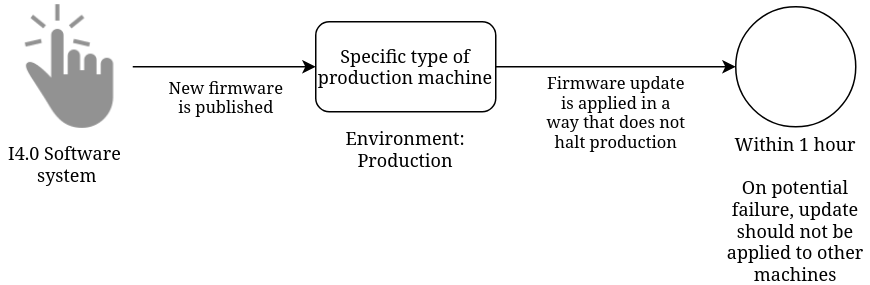
\includegraphics[width=\linewidth]{Images/Availibility.png}
    \caption{Availability Quality Attribute Scenario}
    \label{fig:AQAS}
\end{figure}

Figure \ref{fig:CQAS} show the scenario for software correctness. This scenario is only concerned with identifying faulty bottles, and not the handling of faulty bottles. By limiting it to only identifying, the scenario is more specific, and less broad, meaning a more thorough analysis of the specific attribute an be achieved. At each step of production, there will be a chance of failure. A bottle might be uncleaned or under-poured or a label may be printed crookedly. It is not a question of if that will happen, but rather a certainty that it will happen sometimes. Therefore the system needs to be able to identify faults at each step of the production. Assuming four production steps, if a fault is produced at step 1, that leaves 3 steps, that would still be processed, even though the bottle needs to be discarded anyways, which is money out the windows. Therefore, a part of the QA system will be present after each production step, where an image sensor/ computer vision will scan the bottle, and send data to an image processing service, which will then flag the bottle as either faulty or non-faulty. If a bottle is identified as faulty, the image processing service will publish an alert to a bus. This must be completed before the next production step, as to not waste resources. 

\begin{figure}[h]
    \centering
    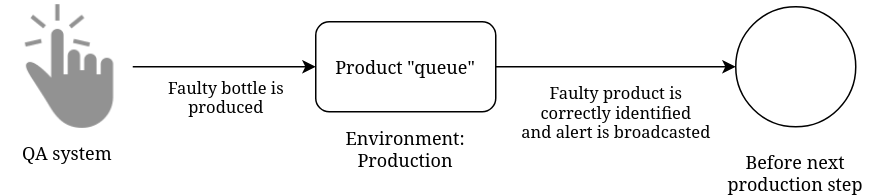
\includegraphics[width=\linewidth]{Images/Correctness.png}
    \caption{Correctness Quality Attribute Scenario}
    \label{fig:CQAS}
\end{figure}


\section{Design}
\label{sec:middleware_architecture}

% Description of the overall architecture designs
% Argue for tactics used to archieve the QASes
% Discuss the trade-offs

This section will describe a proposed design that aims to achieve the stated QAS's mentioned in the previous section.

\subsection{Suggested design}
Our approach to ensuring correctness in our Quality Assurance System, can be outlined in the high-level diagram in figure \ref{fig:high-lvl-corr}.

\begin{figure}[h]
    \centering
    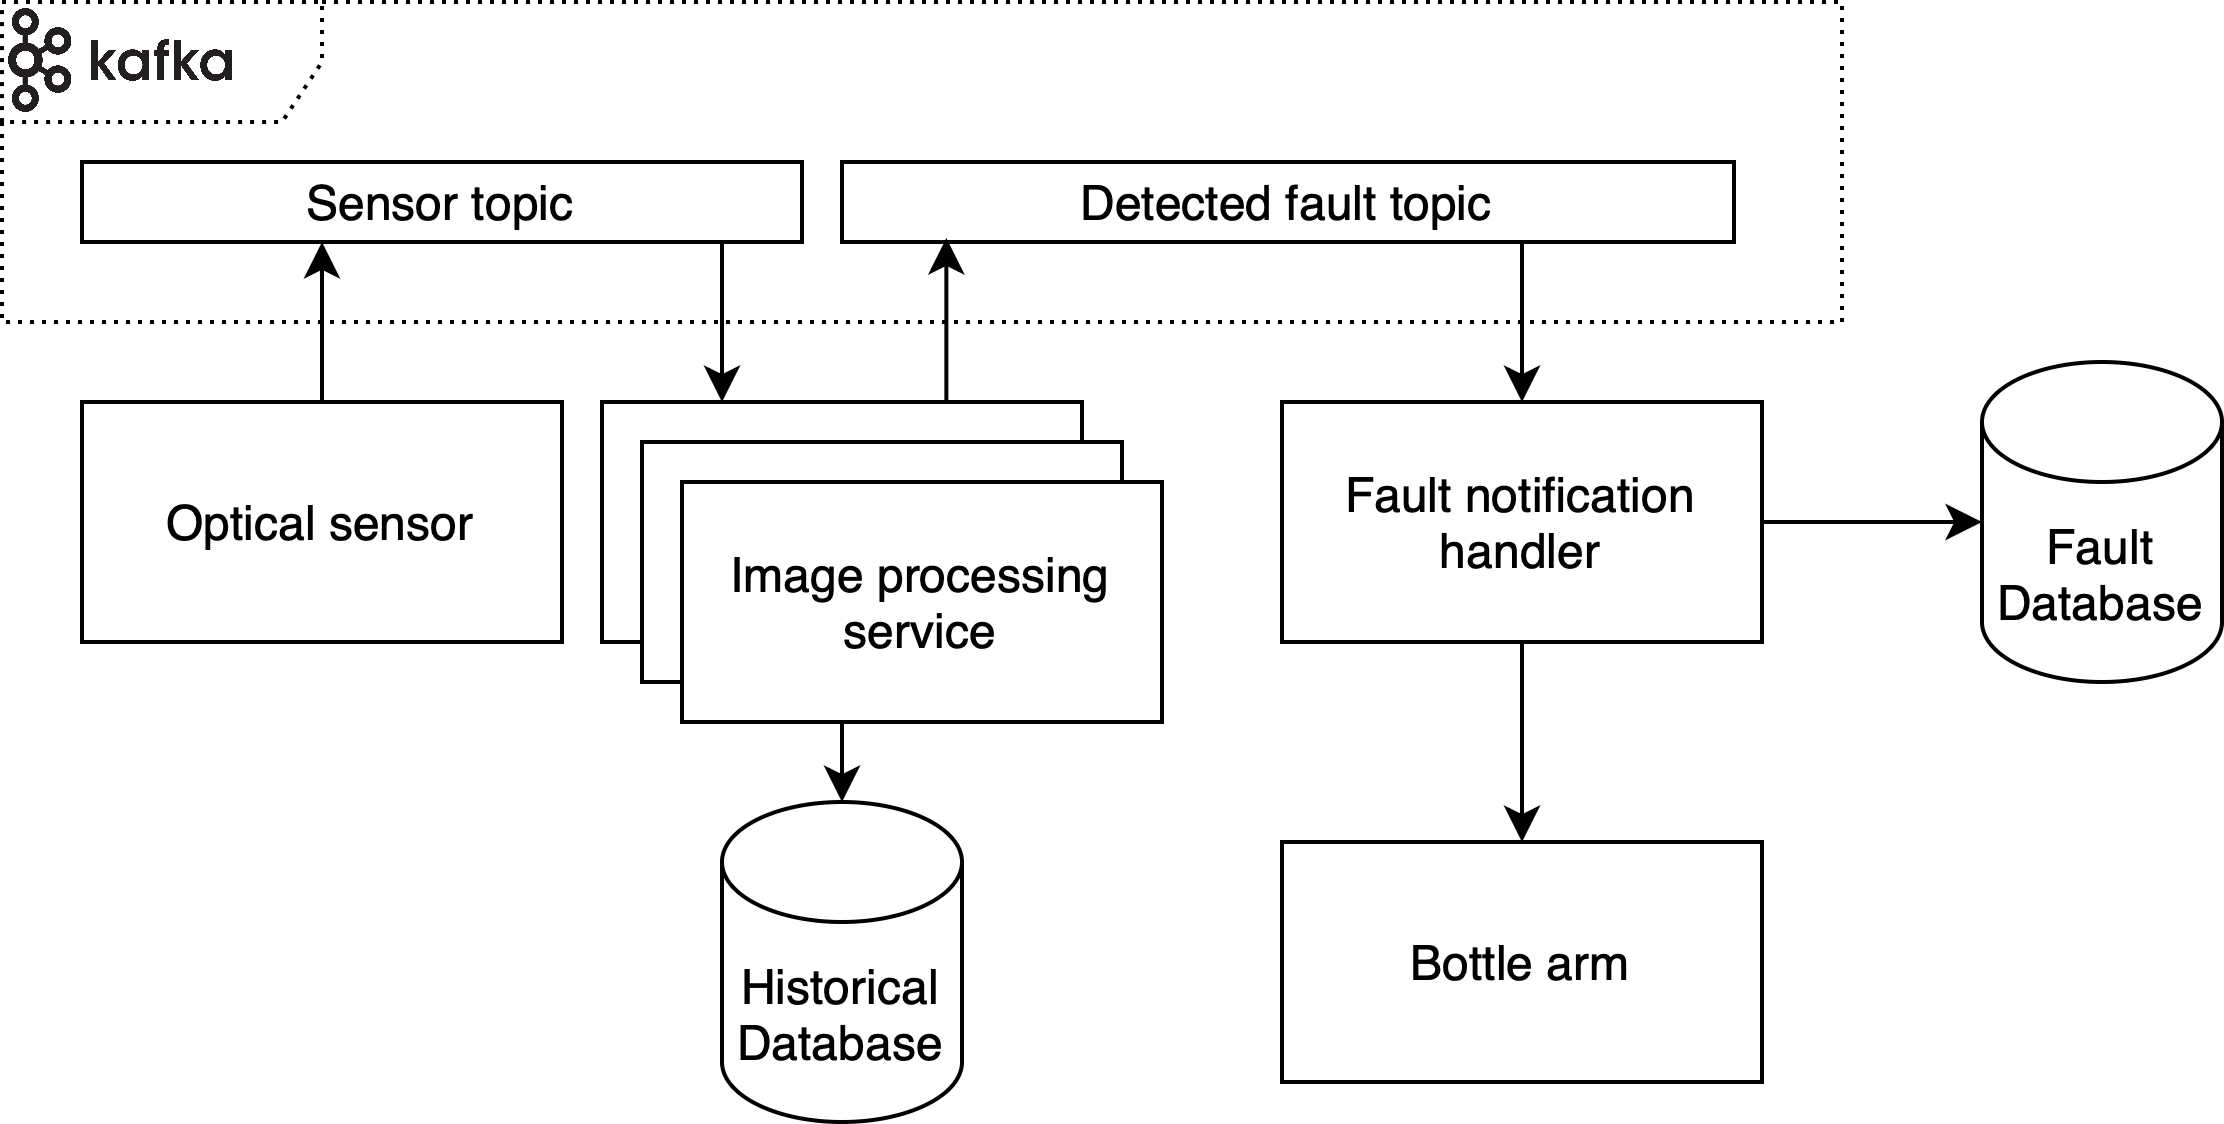
\includegraphics[width=\linewidth]{Images/arkiii.png}
    \caption{High level view of Correctness solution}
    \label{fig:high-lvl-corr}
\end{figure}

At each production step, optical sensors will be placed which will produce images of each bottle. This sensor will then offload data to a topic in a message bus. An image processing service subscribes to the topic and processes the image and saves the image in a database that stores historical data of all bottles. The data stores will be: record id, cleanliness, certainty, imageBlob, sensorID and a timestamp. If the image processing service identifies that the cleanliness is below a certain threshold, it will publish an event to a fault topic, in the message bus. This event will be picked up by a Fault Handling Service, which will notify an arm which will remove the specified bottle. The fault handler will then save a record of the faulty bottle, including why it was removed.

\subsection{Decision points}
This section will describe some of the decision points of the design of the Quality Assurance System


\subsubsection{Joined or split image processing}
The first option that came to mind when designing was to combine the optical sensor and image processing as they are directly related. This would mean minimal latency while minimizing the possibility of data loss between the two components. 

After discussion however, we proposed another solution. Split up the two component, so that the optical sensor is isolated from the image processing service. This idea came from a discussion of what would happen if the processing of an image got stuck, or a service somehow got in a non-functioning state. By having the sensor and image processing joined, failure of one, would render both useless. A small software bug in the image processing would render any images taken by the sensor unprocessed. By separating these two, failure of one, would not impede the other, meaning that a hung process would not cease the optical sensor from doing more readings. 

Another case that was discussed was that what if at full load, the optical sensor would produce more images than a single image processing service could handle. If that was the case, production would have to be forced to slow down manually, so that the requirement of no faulty bottles reaching distribution, is still achieved. If the system is running at full load, we can assume that it has received a large order on a deadline, meaning that slowing down will limit the chances of fulfilling the order in time. 

Instead, by separating the sensor and processing, we allow the sensors to offload data as fast as possible. The sensor should not care to whom it is sending its data, just that it has made a reading, and published it. Then, due to the separation of responsibilities, any instance of the image processing service can subscribe to the topic and process the image. This means that at high system load, the system will be able to scale the amount of image processing service instances to the current load. This could be done by e.g. having a measure of mean time between each finished processing. If the measure goes above the time between each image, it is a sign that current instances are at capacity, and that another instance may be needed. This is just one way however, and effectiveness would have to be tested. 

This decision also allows us to more seamlessly test new versions/models of a computer vision machine learning AI. This way, we can slowly test a new model by limiting the specific version to processing fewer bottles, while keeping other instances on the old version, allowing operators to verify its correctness, with minimal casualties. When data points to the service are performing correctly, more instances of the new model can replace the old version, and when enough data is collected to verify correctness, the old version can be outright replaced. This is also called Canary Deployment\cite{strasser2023evaluation}.

\subsubsection{Persistence strategy}
As the proposed system is a service oriented architecture, that will likely be deployed in a distributed manner, persistence strategies need to be explored. 

Though the system could be defined as distributed, the magnitude of distribution is limited. It would most likely not be distributed across multiple countries and continents, but rather throughout a production facility. 

This limited distribution would technically allow for usage of a single database. This would give the whole system a single source of truth, and provide no consistency issues. Things may however be moving fast in the system, and bottlenecks could appear when using a single database. It could help to think of certain tasks as domains. If the quality assurance system is a larger domain, it could prove useful to imagine imaging and processing as a subdomain for itself, meaning it should own all its related data. 

Fault handling would then be another subdomain, where it would own its related data. This would ensure that a database would only need to perform transactions on domain related data, which should help with database availability. This approach is more resource intensive however, as operating multiple databases simply takes more computing power.
By having a specific fault database, we can easily see the effectiveness of the fault handling system. In the Historical database, we have a record of each bottle that has been through the system, regardless of state. We could for a given time period, say the last 24 hours, pull a set of records and note how many failures have been reported. We can compare this number to the amount of records in the same time period in the fault database. At any given time, this number should be identical. Mismatch would indicate a problem in the production system. If the number in the fault database is lower, it means that faulty bottles are not picked up and discarded, which means that faulty products will reach the customer, which is unacceptable. In this way, operators can observe how their system is performing at all times, namely each single component of the quality assurance system, and the quality assurance system as a whole. Reasons could vary, but could e.g. be the cause of slow image processing resulting in bottles not being flagged as faulty before reaching the end of the production system.

\subsubsection{Messaging}
Due to the interoperability requirement, we knew that a message bus of some kind had to be used. A message bus allows for uncoupled asynchronous event communication as opposed to request/response based communication \cite{inngest2022}. Since the system would have to be applied on different components of the production system, and that once a production step is finished, it simply has to forward the product, not do a "handshake" with the next step, which can be replicated in a software system by using event based communication. This also allows seamless changing of system components, as they are decoupled from other components. As long as components adhere to tailored interfaces, different manufacturers or versions of e.g. sensors can be used. An interface for the image processing service could be that it needs the data exported by the sensor as described earlier, and saves the result, then exports it if the result has been identified as a fault. As long as the service does that, programming language or version is unimportant. A drawback to the event based pub/sub style of communication is also the lack of a handshake. You have no idea if a message has reached a target succesfully, and dropped requests are much harder to accommodate. 

The chosen solution has fallen on a MQTT message bus, as many IOT connected devices already implement the MQTT protocol, which minimizes some responsibilities. Mosquitto was chosen as the bus, because it is an open source project by the eclipse foundation, meaning it has great support. It is also lightweight, and thus suitable for running on embedded devices, which could be necessary in I4.0 systems.

\subsubsection{Databases}

The choice of database(s) for historical and fault data is based on several key features of their respective requirements. Because they have different purposes, they have different implementations. We have chosen NoSQL for both databases, because they generally are faster for read/write operations, and since we wont be making many SELECT statements during production hours, it is the obvious choice for many small key/value writes. For the fault database, we have employed a classic MongoDB database for scalable and ACID compliant storage of key/value entries. ACID compliance ensures fault tolerance and data durability, which states that even in case of system failure, data will not be lost in transaction. Due to the fact that this is a NoSQL database, we are in the same realm as the database for historical data, for which we have chosen BangDB. It is also a NoSQL, ACID compliant database for key/value entries. It is optimized for things like live time-series data, with built-in tools for visualizing the data in graphs, making AI research like Machine Learning on the data and/or running statistics for end of day/week/month/year analysis.
\section{Evaluation}
\label{sec:evaluation}
This Section describes the evaluation of the proposed design.
Section \ref{sec:design} introduces the design of the experiment to evaluate the system. 
Section \ref{sec:measurements} identifies the measurements in the system for the experiment.
Section \ref{sec:pilot_test} describes the pilot test used to compute the number of replication in the actual evaluation. 
Section \ref{sec:analysis} presents the analysis of the results from the experiment. 

\subsection{Experiment design}
\label{sec:design}
The experiment will test the correctness quality attribute of the QA system, which is also tightly constrained to the availability QA, meaning that the software for each production system has to perform its own task correctly, without hindering the rest of the production system. 
This experiment is only run on the cleaning service, meaning bottles are only checked for cleanliness, and not the rest of the multitude of things that could go wrong.

\subsubsection{Selected QA} 
The QA system must be able to correctly identify bottles that are not thoroughly cleaned at a rate of \textgreater 99.9\%.

\subsubsection{Experiment process}
\begin{itemize}
    \item The Optical sensor scans a bottle and publishes the data to an MQTT topic.
    \item An image processing service subscribes to the topic, interprets the result. If the result is a faulty bottle, another topic is notified, so that a fault handling service can remove the entity from the production system.
    \item Regardless of the result, it is persisted in a database, so that we have historical data of how correctly the system is functioning. Images will be stored in the database as blobs for future reference and to potentially help train an AI to assist with the image processing. Saved data will include a unique record id, cleanliness percent, certainty, imageBlob, sensorID and a timestamp.
    \item The fault handling service removes the bottle from the production system, and persists the bottle, image blob, and reason for removal (in this experiment, only unclean). 
\end{itemize}

\subsubsection{Metadata}

\begin{itemize}
    \item \textbf{RecordID: }A specific record should be unique and traceable. Having an id for each record ensures this.
    \item \textbf{Cleanliness percent: }Will show a number of how clean a bottle is analyzed to be. Allows operators to identify specific machines that may averagely, clean worse than others, allowing them to adjust settings and optimize parameters.
    \item \textbf{Certainty: } Will express how certain an image processing service is of its cleanliness percent. Could be used to provide a measure of how precise a version of a potential ML library is, or whether external parameters, like lighting, around sensors are sub-optimal.
    \item \textbf{ImageBlob: } A blob object of the image, allowing for retraining of an ML AI.
    \item \textbf{SensorID: } The ID of the sensor which produced the image, allowing operators to identify specific sensors which might be operating sub-optimally.
    \item \textbf{Timestamp: } A timestamp of when the sensor made its observation. Allows operators to pull data in a specific time-frame, which can be used to identify performance of specific periods, which can be used to optimize future production.
    \item \textbf{Removal Reason: } (in a full environment) could be used to identify which fault happen the most.
\end{itemize}


\subsection{Measurements}
\label{sec:measurements}
\subsubsection{Measurement selection}
This experiment will measure the percentage of uncleaned bottles, which are not caught by the image detection system. This percentage must be \textgreater99.9\% for the experiment to be a success. In reality, only relying on correctness is not feasible. As the QA system \emph{cannot} be a hindrance to the rest of the production system to satisfy the availability requirement, it put a severe performance requirement on the image processing service. A bottle must be identified clean or unclean, with time to spare until the next production step, such that it can be removed \emph{before} the next production step. As described in section \ref{sec:middleware_architecture}, Solution, possible bottlenecks have been addressed by separating the optical sensor, and the image processing service by using a sensor topic of a message bus. In this way, image processing could be scaled independently of the optical sensors. In a real setting, that means, that the test would likely also measure computation time of each task, to evaluate service efficiency. In this way, different versions of the image processing service could also be tested, by supplying a set of pre-identified bottles, and running them through different versions of the image processing, to see if one version is better at identifying faults than another. When running this version of the experiment, which follow the exact same procedure, the measurement instead becomes the correctness of the image-processor instead of the fault handler.

\subsubsection{Justification}
In this mock environment, a random chance could decide the time it takes to "make a calculation" of whether a bottle is clean or not, to emulate that a task may not be completed with time to spare to next step. It was however decided, that this simply did not make sense in the mock environment. A random chance would not improve the usefulness of the experiment, it would just occasionally show a wrong result. The experiment is emulating image processing in a single production step, and as such, time is not a factor. A parameter that could be introduced to emulate some variability, is a certainty parameter, that could provide the possibility of discarding bottles where the sensor is simply too uncertain. This could spark a discussion of what tolerance operators should have, around certainty. Is it better to discard bottles, when certainty is below a threshold, or do we trust the system enough, to take the chance when certainty is low. It could also be used to emulate a new AI ML model, which could be a good reason to run a correctness experiment in a real environment. However due to time constraints, the uncertainty parameter has been left out of the experiment design

As such, the experiment will only include the amount of bottles produced, amount of faulty bottle produced, and the amount of faulty bottle that have been discarded.

\subsection{Pilot test}
\label{sec:pilot_test}

The system designed for this experiment consists of:
\begin{itemize}
    \item An optical sensor
    \item Image processing service with underlying database
    \item A fault handling service
    \item A message bus
\end{itemize}
The process follows:
\begin{enumerate}
    \item The optical sensor publishes the data of the bottle it has just cleaned to a MQTT Topic. The data is synthetic, and consists of sensorID, sensorData, bottleID, and a timestamp. The sensor data is a number between 0-100, and any number under 10, should be categorized as a faulty (unclean) bottle
    \item The “image processing” service subscribes to the before mentioned topic, and takes the most recent, non processed  entry, meaning MQTT is set to “Exactly Once” handling. The image processor then analyzes the data and evaluates whether the sensorData attribute is 10 or under. If it is, it publishes the bottleID and sensorID to a “fault” MQTT topic. Regardless of the cleanliness of the bottle, data is persisted in a historical database.
    \item The fault handling service subscribes to the “fault” topic, and as soon as it gets a new event, consisting of the bottleID, and sensorID, the bottle is removed from the production systems, such that it is not distributed to customers. The reason for including a sensorID, is to enable the ability to identify sensors which publish more faulty bottles than others. This could be due to a variety of things, like faulty sensors. It could also be used to optimize the production line in the future, if certain parts of the line are more faulty than others.
    \item Ideally, all the bottles would have to go further down the production system, for the next step in the production, so that we can verify that a faulty bottle does not reach the next step, when identified as faulty. We have however not designed this part of the system yet.
\end{enumerate}

The experiment is started by the C++ Publisher, which emulates the optical sensor, and the size of the experiment can be set by setting the amount of bottles that should be processed, and how frequently they should appear.

For the pilot test, we chose a sample size of 10.000, which provides us a sufficient size to evaluate correctness of our QA system



\subsection{Result analysis}
\label{sec:analysis}
%data analysis and interpretation
A total of three experiments were run, to ensure that there is enough data to extensively analyze the results.\\
The results of our first experiment can be summed up as follows:
\begin{table}[h]
    \centering
    \caption{Experiment I results}
    \begin{tabular}{lr}
        \toprule
        \textbf{Description} & \textbf{Value} \\
        \midrule
        Size & 10,000 \\
        Entries in Historic Database & 9,395 \\
        Entries tagged as clean & 8,470 \\
        Entries tagged as unclean & 925 \\
        Entries detected by fault system & 925 \\
        \bottomrule
    \end{tabular}
    \label{tab:ExpI}
\end{table}
\\
From the first results, as seen in table \ref{tab:ExpI}, of our experiment described in section \ref{sec:pilot_test}, we can identify that our fault detection system is, in terms of our measurement, operating correctly, and that all faulty bottles have been identified and handled, meaning that no faulty bottles will reach the consumer. We can however also identify a rather large problem in this first test-run. Of our sample size of 10.000, only 9395 of those samples are persisted in the historic database, meaning there is a drop of 605 samples which tells us that somewhere in the process we lose about 6\% of our data. Due to this error rate, we adjusted some parameters, including making sure that the publisher would wait for the mysql database to be healthy, by also including a health check in the docker compose. After this, we ran the experiment 2 more times. 
\\\\
The results of our second experiment can be seen in table \ref{tab:ExpII}:
\begin{table}[h]
    \centering
    \caption{Experiment II results}
    \begin{tabular}{lr}
        \toprule
        \textbf{Description} & \textbf{Value} \\
        \midrule
        Size & 10,000 \\
        Entries in Historic Database & 9993 \\
        Entries tagged as clean & 8967 \\
        Entries tagged as unclean & 1026 \\
        Entries detected by fault system & 1026 \\
        \bottomrule
    \end{tabular}
    \label{tab:ExpII}
\end{table}
\\\\
The results of our third experiment can be seen in table \ref{tab:ExpIII}:
\begin{table}[h]
    \centering
    \caption{Experiment III results}
    \begin{tabular}{lr}
        \toprule
        \textbf{Description} & \textbf{Value} \\
        \midrule
        Size & 10,000 \\
        Entries in Historic Database & 9989 \\
        Entries tagged as clean & 9004 \\
        Entries tagged as unclean & 985 \\
        Entries detected by fault system & 985 \\
        \bottomrule
    \end{tabular}
    \label{tab:ExpIII}
\end{table}
\\\\
%system performance evaluation
%Quality assurance and data integrity
Looking at the data we received from the first run of the experiment and compare that data to the results of the second and third experiment, we can see a clear difference in entries in the historic database. 
The lack of entries in the historic database in the first experiment is something we see in a much lower degree in further tests of the experiment and we can exclude the possibility of the publisher not publishing 10.000 entries, as we made sure to include a counter that the producer would announce. Along with this, the amount of published messages could also be verified by by our logging. For testing purposes we made sure to log each and every message to be published in a format like in listing \ref{lst:log}.
    
\begin{lstlisting}[label=lst:log, caption=Logging format for verification]
n=1 ...
2. {"data": "84", "sId": "3..", "t": "2."}
2. {"data": "39", "sId": "u..", "t": "2."}
2. {"data": "46", "sId": "N..", "t": "2."}
2. {"data": "3",  "sId": "o..", "t": "2."}
2. {"data": "94", "sId": "j..", "t": "2."}
2. {"data": "27", "sId": "z..", "t": "2."}
2. {"data": "43", "sId": "i..", "t": "2."}
... n=10.000
\end{lstlisting}

The first \textit{"2."} is a timestamp made by our logger. The \textit{sensorData} field (shortened to \textit{data}) shows the cleanliness of the bottle. The \textit{sensorID} (shortened to \textit{sId}) shows the "sensor" that produced the image. The \textit{timestamp} (shortened to \textit{t} shows the sensor-registered time at image production. Verification was as simple as filtering the logs, copying, and pasting them in a text editor and verifying the amount of line, which counted to 10.000.
We can also conclude, that the issue is not with the fault handler, as it has the same amount of entries, as the subscriber has amount of identified faults. That means, that the error in regard to the entries in the historic database in the first test is likely located between the publisher, subscriber and database.



The rest of the logged data in the tests largely mimic each other. We can see that the test results show a high level of similitude and there aren't any issues with faulty bottles not being registered. For all three tests every unclean bottle in our database, gets caught by the fault detection system and thus our goal of creating a system that detects \textgreater99.9\% of the faulty bottles is met.

Because the data in all three tests are so similar, we can also be fairly certain that these tests aren't just lucky outliers that just happens to coincidentally prove that our system works. The similarity helps assert the data as consistent and also underlines that the system is reliable when it comes to registering and handling faulty bottles.

For good measure and to establish absolute certainty that our system works as intended, we decided to run an alternative experiment on the second form of measurement as described in section \ref{sec:measurements}, where the system instead measures the correctness of the image processor. To do this, a predefined array of bottle objects were created, consisting of 50 bottles, 11 of which were faulty. The publisher was then modified to read from this array, instead of produce new bottles. This experiment yielded the results shown in table \ref{tab:AltExp}.

To further support data from the previous tests, we see that this test proves that the image processor works as intended as the predefined 11 faulty bottles were all tagged as unclean. But in contrary to the previous experiments all 50 of our entries were recorded in the alternate experiment. The disappearing data issue from the first experiments is no longer present, so lets dive into why that is.
\begin{table}[h]
    \centering
    \caption{Alternate Experiment Result}
    \begin{tabular}{lr}
        \toprule
        \textbf{Description} & \textbf{Value} \\
        \midrule
        Size & 50 \\
        \hline
        Predefined clean & 39 \\
        Predefined faults & 11 \\
        \hline
        Entries tagged as clean & 39 \\
        Entries tagged as unclean & 11 \\
        Entries detected by fault system & 11
        \bottomrule
    \end{tabular}
    \label{tab:AltExp}
\end{table}

%Tålmodighed når man opretter et topic fordi den er langsom (Kan være en grund til "missing inpunt in historic database")
The team decided to comb through previous data, realizing, that the logs would show the publisher publishing before it would log the "Connected" message, signifying a connection to the MQTT bus and topic, which could mean that the publisher was trying to publish messages before the topic was ready. A simple way to test this was to "sleep" the thread for a short amount of time, before publishing. Doing this yielded the desired results and 100\% of the data would be recorded in the historic database. Even though "sleeping" the thread yielded the proper results, observing the data shown in the first 3 experiments, \ref{tab:ExpI}, \ref{tab:ExpII} \& \ref{tab:ExpIII}, still shows that the test results mirror the results of the alternate experiment \ref{tab:AltExp}, where the entirety of the data got processed.

Although we located the fault that caused some of the data to be lost, it is worth referring back to our second research question, to emphasize that running a distributed system like ours brings a necessary trade off. This trade-off being that it is more difficult to locate where faults arise because there are more points of failure. And it shows in our work as well, because it took us more than three test-runs of the experiment to realize why some of the data got lost.
\section{Future work}


As our experiment showed, somewhere along the testing of our system irregularities occurred. The experiment proves that there is room for improvements. Notably we experienced missing requests/objects in the historic database, which was identified to be caused by a non-ready MQTT bus/topic. This is a clear indicator of a place where a heartbeat or health-check could be used. Currently, the solution is to wait two and a half seconds before beginning to publish messages. This is however unreliable as it is not guaranteed to be ready in that amount of time. The publisher should wait until the MQTT bus/topic reports that it is ready either passively (heartbeat) or actively (health-check). 

Obvious future work lies in applying learned principles here to the rest of the production system. The image processing and fault handling is built on principles that ensure high availability and interoperability while allowing for easy scaling meaning the QA system should be easily applicable to other parts of the system. 

Next steps include: the label printer, bottle filler and the bottle capper. 

Another thing that could be worked on, is actual image processing. While the producer system is more of a proof-of-concept setup, the experiments we conducted could actually be used to measure a whole load of measurements. Future work could include comparing different versions or models. Or it could be used to compare different image processing frameworks/libraries or even implementation in different languages, measuring for processing speed and correctness. Generally, the experiment design allows for testing for a multitude of things, depending on which part is exchanged. The setup created could be treated as a baseline, as it has been proved to work as intended. It could be interesting to test whether Kafka could be used instead of or along side MQTT, as it handles being distributed really well. The experiment could vary with what velocity and size data is published, to see which bus handles different sizes best. Databases could also be tested for performance and scalability by also varying the before-mentioned properties of transmitted data   

The CI/CD pipeline is also incredibly limited, and is currently more in a state of "this could be used" than actually ready to use. Implementing a fully working CI/CD pipeline is high on the priority list of future work.


\section{Conclusion}

In this report, we have described the process of creating an architecture for an industry 4.0 production system producing bottled beer. To solve such a  challenge, we have created and proposed a service oriented distributed solution, to comply with general industry 4.0 quality attributes which are availability, interoperability and deployability. By using a service oriented architecture, individual services can be updated without disturbing others using different strategies, and can also be implemented in different languages, as long as the comply with predefined interfaces. The distributed nature allows routing production away from potential unavailable components of the production system. Trade-offs in the system come in forms of complexity. Running in a distributed way also means more machines, which means more operational complexity. Generally when computation is spread out, it opens more fault surfaces. Often however, the magnitude of each fault surface is reduced. As out experiments showed, our solution fulfills the requirements of our system and our most important quality attribute which is correctness.

\bibliographystyle{IEEEtran}
\bibliography{references}
\vspace{12pt}
\end{document}
